\thispagestyle{hoccungpinone}
\pagestyle{hoccungpi}
\everymath{\color{hoccungpi}}
\graphicspath{{../hoccungpi/pic/}}
\blfootnote{$^{1}$\color{hoccungpi}Lớp $12$ Toán $1$, Trường THPT Amsterdam, Hà Nội.}
\blfootnote{$^{2}$\color{hoccungpi}Khoa Toán -- Tin, Đại học Sư Phạm Hà Nội.}
\begingroup
\AddToShipoutPicture*{\put(0,616){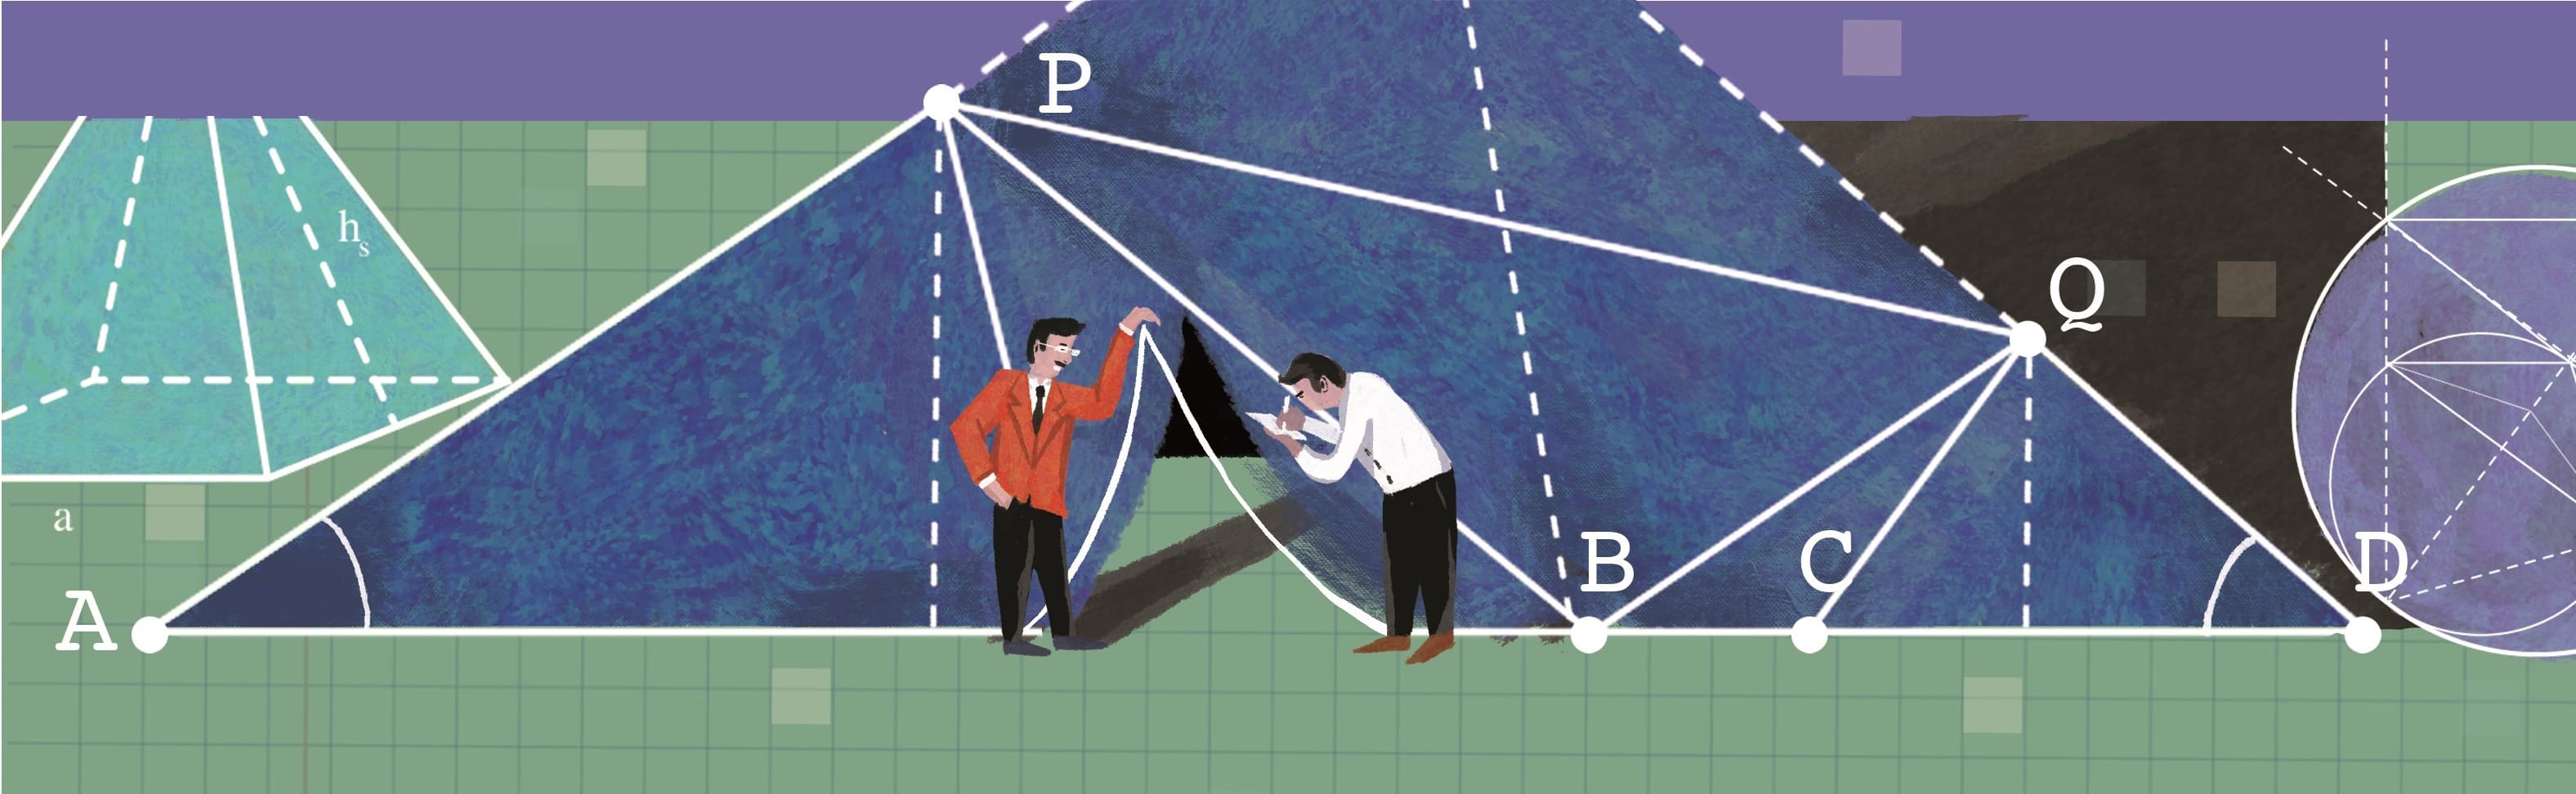
\includegraphics[width=19.3cm]{../bannerhoccungpi}}}
\AddToShipoutPicture*{\put(80,550){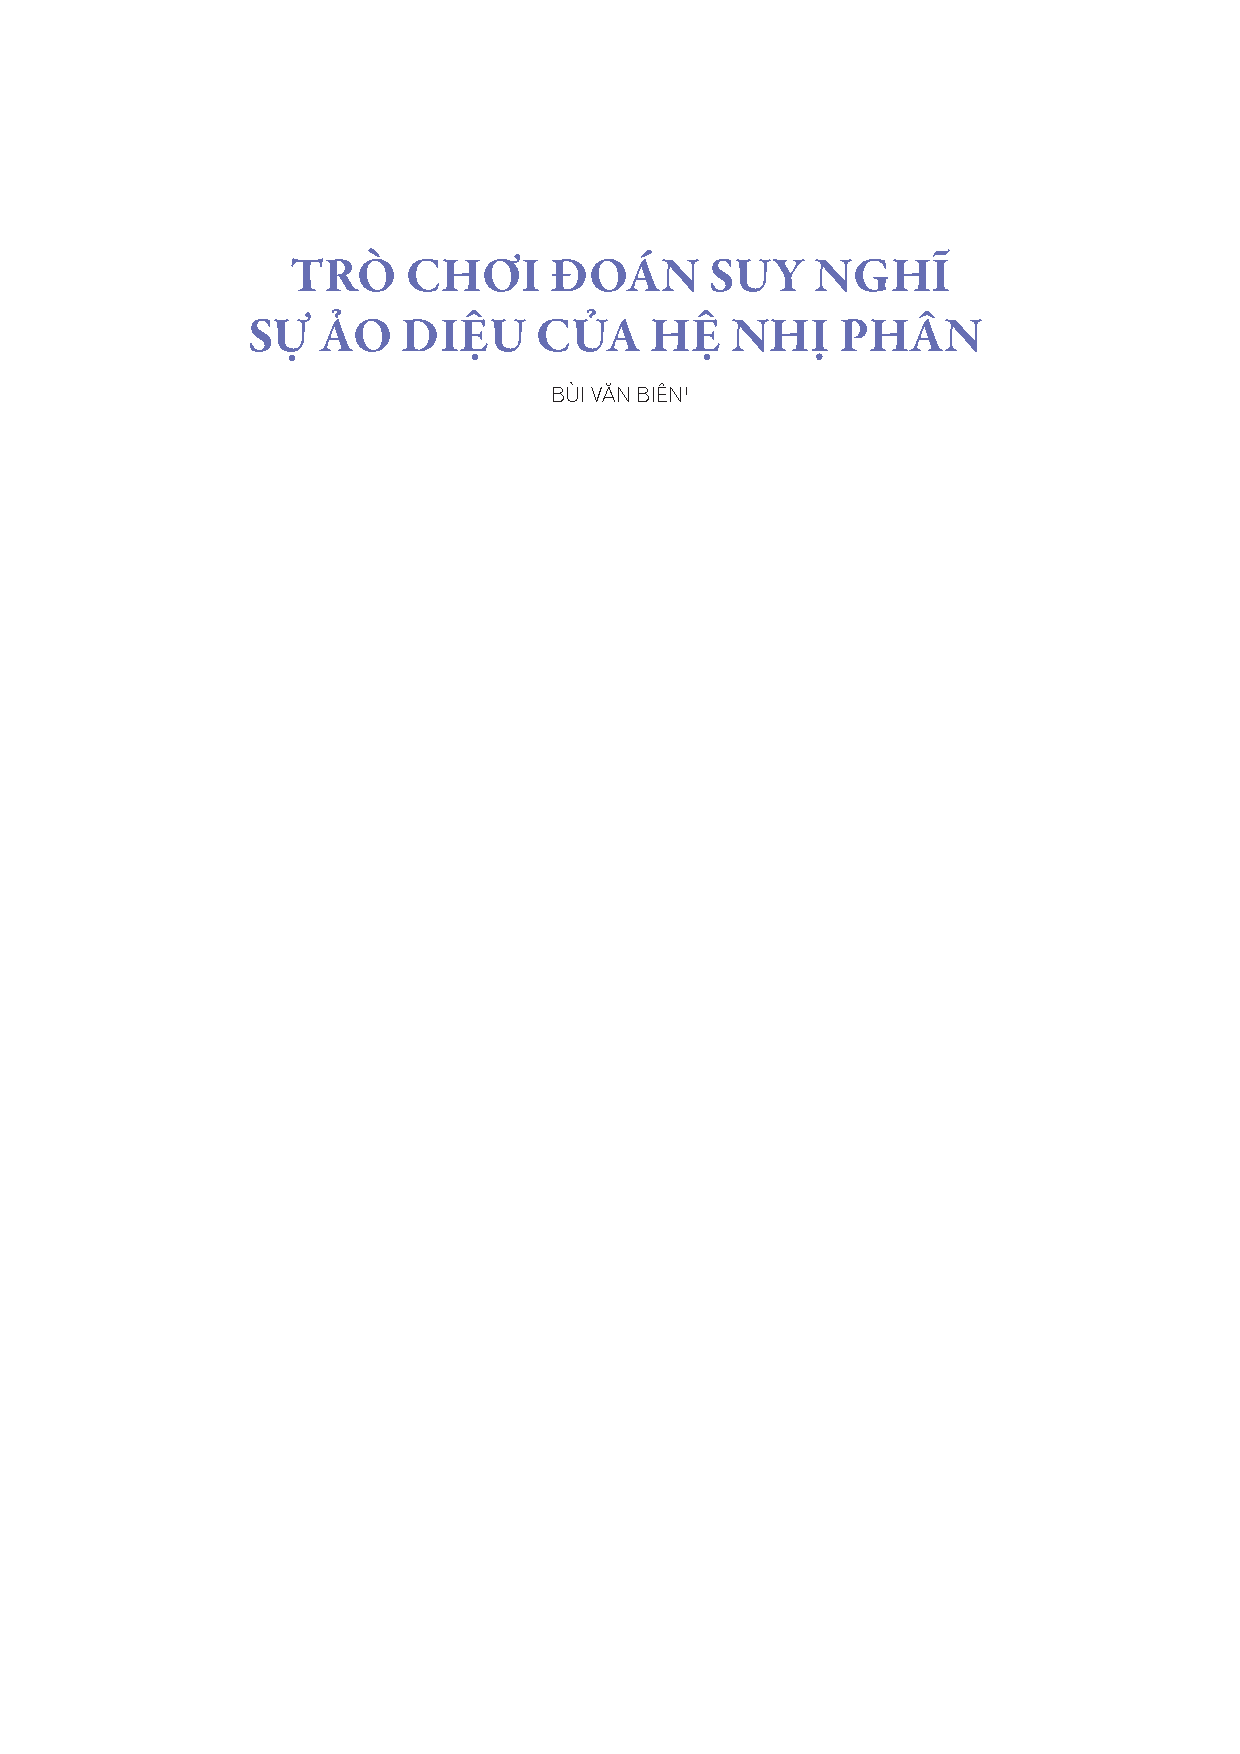
\includegraphics[scale=1]{../tieude1.pdf}}}
\centering
\endgroup

\vspace*{160pt}

\begin{multicols}{2}
$\pmb{1.}$ \textbf{\color{hoccungpi}Giới thiệu}
\vskip 0.1cm
Định lý Fermat lớn nói về sự không tồn tại bộ ba số nguyên $a,b,c$ khác $0$ sao cho $a^n+b^n=c^n$ với $n\ge 3$ là số nguyên dương, đã được Andrew Wiles [$5$] chứng minh vào năm $1995$, nhưng ít ai biết rằng có một định lý ``Fermat" tương tự cho đa thức đã được chứng minh trước đó hàng chục năm trước, tức không tồn tại ba đa thức $f(x),g(x),h(x)$ với hệ số thực, ít nhất một đa thức khác đa thức hằng, đôi một không có nghiệm chung sao cho $f(x)^n+g(x)^n=h(x)^n,$ với $ n\ge 3$ là một số nguyên dương cho trước.
\vskip 0.1cm
Định lý Fermat cho đa thức là hệ quả của Định lý Mason -- Stothers, đầu tiên được Stothers [$4$] chứng minh vào năm $1981$, và Mason [$3$] độc lập phát hiện ra sau đó ít lâu. Các chứng minh đó nhìn chung là phức tạp, không sơ cấp. Năm $2000$, Snyder [$2$] đã đưa ra một chứng minh mới, chỉ với các kiến thức toán phổ thông cho định lý này. Trong bài viết này, chúng tôi giới thiệu chứng minh của Snyder và sau đó áp dụng Định lý Mason--Stothers để chứng minh Định lý Fermat cho đa thức và một số kết quả liên quan khác.
\vskip 0.1cm 
$\pmb{2. }$ \textbf{\color{hoccungpi}Định lý Mason -- Stothers}
\vskip 0.1cm
	\textbf{\color{hoccungpi}Định lý} $\pmb{1}$ (Mason -- Stothers)\textbf{\color{hoccungpi}.} 
\textit{	Cho $a(x),$ $b(x)$ và $c(x)$ là các đa thức khác đa thức hằng, với hệ số thực, đôi một không có nghiệm phức chung và thỏa mãn: $a(x) + b(x) = c(x)$. Khi đó
	\begin{align*}
		\deg(c) \le n_0{(abc)} - 1,
	\end{align*}
	trong đó ta ký hiệu $n_0(f)$ là số nghiệm phức phân biệt của đa thức $f(x)$ và $\deg(f)$ là bậc của đa thức $f(x).$}
	\vskip 0.1cm
	Để chứng minh Định lý này, ta cần Bổ đề sau:
	\vskip 0.1cm
	\textbf{\color{hoccungpi}Bổ đề} $\pmb{1.}$
	\textit{Cho $f(x)$ là một đa thức với hệ số thực, khác đa thức $0$.  Khi đó,
	\begin{align*}
		\deg(f) \le \deg(f,f') + n_0(f),
	\end{align*}
	trong đó ta ký hiệu $(f,f')$ là ước chung lớn nhất của hai đa thức $f(x)$ và $f'(x)$ ($f'(x)$ là đa thức đạo hàm của đa thức $f(x)$).} 
	\vskip 0.1cm
	\textit{Chứng minh.}
	Gọi $\alpha_1, \alpha_2, \ldots,  \alpha_m $ là các nghiệm phức phân biệt của $f(x)$ với các bội $a_1, a_2, \ldots , a_m$ tương ứng. Khi đó, ta có phân tích
	\begin{align*}
		f(x) \!=\! a(x \!-\! \alpha_1)^{a_1}(x \!-\! \alpha_2)^{a_2}\ldots (x \!-\! \alpha_m)^{a_m},
	\end{align*}
	với $a\in \mathbb{R}$ và $a_1+a_2+\cdots+a_m=\deg f(x).$
	Ta có, theo công thức Leibniz, đạo hàm của $f(x)$ được cho bởi:
	\begin{align*}
		&f'(x) \\
		=\,\,& aa_1(x - \alpha_1)^{a_1-1}(x - \alpha_2)^{a_2} \ldots (x - \alpha_m)^{a_m}  \\
		&\!+  a(x - \alpha_1)^{a_1} [(x - \alpha_2)^{a_2}\ldots(x - \alpha_m)^{a_m}]'.
	\end{align*}
	Suy ra, với mỗi $i=1, 2, \ldots, m$, đa thức $(x-\alpha_i)^{a_i-1}$ cùng là ước của $f(x)$ và $f'(x)$.
	Do đó 
	\begin{align*}
		&(x - \alpha_1)^{a_1 - 1}(x - \alpha_2)^{a_2 - 1} \ldots \\
		&(x - \alpha_m)^{a_m - 1} \mid (f,f').
	\end{align*} 
	Vì $f(x)$ là đa thức khác đa thức hằng nên $f'(x)$ khác đa thức $0$ và do đó $(f, f')$ cũng khác đa thức $0$. Suy ra
	\begin{align*}
		&\deg((x - \alpha_1)^{a_1 - 1}(x - \alpha_2)^{a_2 - 1}\ldots \\
		&(x - \alpha_m)^{a_m - 1}) \leq \deg(f,f'),
	\end{align*} 
	hay 
	\begin{align*}
		&(a_1-1)+(a_2-1)+\cdots+(a_m-1)\\
		\leq \,&\deg (f,f').
	\end{align*}
	Suy ra
	\begin{align*}
		\deg(f) - n_0(f) \leq \deg(f,f').
	\end{align*}
	Vậy bổ đề được chứng minh
	\vskip 0.1cm
	\textit{Chứng minh Định lý} $1.$
	Từ giả thiết 
	\begin{align*}
		a + b = c, \tag{$1$} 
	\end{align*}
	bằng cách lấy đạo hàm hai vế, ta được
	\begin{align*}
		a' + b' = c'. \tag{$2$}
	\end{align*}
	Nhân ($1$) với $a'$ và nhân ($2$) với $a$ và trừ vế với vế, ta được
	\begin{align*}
		a'b - ab' = a'c - ac'.
	\end{align*}
	Suy ra $(a,a'), (b,b')$ và $(c,c')$ đều là ước của $a'b - ab'$.
	\vskip 0.1cm
	Do các đa thức $a,b,c$ đôi một không có nghiệm phức chung nên các đa thức $(a,a'), (b,b')$ và $(c,c')$ cũng đôi một không có nghiệm phức chung. Suy ra
	\begin{align*}
		(a,a')(b,b')(c,c') \mid a'b - ab'.
	\end{align*}
	Hơn nữa, ta có $a'b - ab'\ne 0$. Thật vậy, nếu $ a'b - ab'= 0$ thì $\left(\dfrac{a}{b}\right)'=0$ hay $\dfrac{a}{b}$ là hằng số. Do đó $a$ và $b$ có nghiệm chung (mâu thuẫn với giả thiết).
	Vì vậy, 
	\begin{align*}
		\deg ((a,a')(b,b')(c,c'))\leq \deg(a'b - ab').
	\end{align*} 
	Mặt khác, hiển nhiên ta có 
	\begin{align*}
		\deg(a'b-ab')&\leq \max\{\deg(a'b),\deg(ab')\}\\
			&=\deg(a)+\deg(b)-1.
	\end{align*}
	Vì thế,
	\begin{align*}
		&\deg(a,a') + \deg(b,b') + \deg(c,c') \\
		\leq \,&\deg(a) + \deg(b) - 1.
	\end{align*}
	Chuyển vế bất đẳng thức này và cộng với $\deg (c)$ vào hai vế, ta được 
	\begin{align*}
		\deg(c) \leq& \deg(a) - \deg(a,a') + \deg(b) \\
		&\!\!\!-\! \deg(b,b') \!+\! \deg(c) \!-\! \deg(c,c')\!-\!1.
	\end{align*} 
	Cuối cùng, áp dụng Bổ đề $1$, ta có:
	\begin{align*}
		&\deg(a) - \deg(a,a') \leq n_0{(a)},\\
		&\deg(b) - \deg(b,b') \leq n_0{(b),}\\
		&\deg(c) - \deg(c,c') \leq n_0{(c)},
	\end{align*}
	Từ đó suy ra 
	\begin{align*}
		\deg(c) &\le n_0{(a)} + n_0{(b)} + n_0{(c)} - 1 \\
		&= n_0{(abc)} - 1.
	\end{align*}
	$\pmb{3.}$ \textbf{\color{hoccungpi}Định lý Fermat cho đa thức}
	\vskip 0.1cm
	Áp dụng Định lý Mason -- Stothers, chúng ta có một số kết quả đáng lưu ý. Trước hết, ta có kết quả sau đây:
	\vskip 0.1cm
	\textbf{\color{hoccungpi}Định lý} $\pmb{2}$  (Davenport [$1$])\textbf{\color{hoccungpi}.} \textit{Cho $f(x),g(x)$ là các đa thức với hệ số thực, khác đa thức hằng, đôi một không có nghiệm phức chung. Đặt $h(x)=(f(x))^3-(g(x))^2$ và giả sử $h(x)$ khác là đa thức $0$. Khi đó, $\deg (f) \leq 2\deg (h)-2$.}
	\vskip 0.1cm
	\textit{Chứng minh.}
	Do $f(x)$ và $g(x)$ là các đa thức không có nghiệm chung và $h = f^3 - g^2$ nên $h, f^3$ và $g^2$ đôi một không có nghiệm chung.  Áp dụng Định lý Mason -- Stothers cho ba đa thức $ g^2, h$ và $f^3,$ ta có:
	\begin{align*}
		\deg(f^3) \leq n_0{(g^2hf^3)} - 1,
	\end{align*}
	hay 
	\begin{align*}
		3\deg (f)\leq n_0{(ghf)}-1\leq \deg(ghf) - 1.
	\end{align*}
	Mà $\deg(ghf)= \deg(g) + \deg(h) +\deg(f)$, nên 
	\begin{align*}
		&3\deg(f)\\
		\leq \, &\deg(g) + \deg(h) +\deg(f)-1. \tag{$3$}
	\end{align*}
	Chứng minh tương tự, ta có:
	\begin{align*}
		&2\deg(g) \\
		\leq \, &\deg(g) + \deg(h) +\deg(f) - 1.\tag{$4$}
	\end{align*}
	Kết hợp ($3$) và ($4$), ta được
	\begin{align*}
		&3\deg(f) + 2\deg(g) \\
		\leq \,&2(\deg(g) + \deg(h) +\deg(f) - 1)
	\end{align*}
	hay $\deg(f) \leq 2\deg(h) - 2.$ Ta có điều phải chứng minh.
	\vskip 0.1cm
	\textbf{\color{hoccungpi}Hệ quả} $\pmb{1.}$
	\textit{Không tồn tại hai đa thức với hệ số thực $f(x)$ và $g(x)$, khác đa thức hằng sao cho $f^3-g^2$ là đa thức hằng khác đa thức $0$.}
	\vskip 0.1cm
	Như đã đề cập đến trong phần đầu của bài viết, định lý Mason--Stothers có thể được sử dụng để chứng minh phiên bản đa thức của định lý Fermat lớn.
	\vskip 0.1cm
	\textbf{\color{hoccungpi}Định lý} $\pmb{3}$ (Định lý Fermat cho đa thức)\textbf{\color{hoccungpi}.} \textit{Với mọi nguyên $n\ge 3$, không tồn tại ba đa thức $f(x),g(x),h(x)$, với hệ số thực, đôi một không có nghiệm phức chung, trong đó ít nhất một đa thức khác đa thức hằng, sao cho $f^n+g^n=h^n$.}
	\vskip 0.1cm
	\textit{Chứng minh.}
	Giả sử ngược lại, $f^n+g^n=h^n$. Áp dụng định lý Mason--Stothers cho $3$ đa thức $f^n, g^n$ và $h^n$, ta có:
	\begin{align*}
		&\max\{\deg(f^n), \deg(g^n), \deg(h^n)\} \\
		\le\, &n_0{(f^ng^nh^n)} - 1 = n_0{(fgh)} - 1 \\
		\le\, &\deg(f) + \deg(g) + \deg(h) - 1.
	\end{align*}
	Để ý rằng
	\begin{align*}
		&\dfrac{n}{3}(\deg(f) + \deg(g) + \deg(h)) \\
		=    \,&\dfrac{1}{3}(\deg(f^n) + \deg(g^n) + \deg(h^n)) \\
		\le\,& \max\{\deg(f^n), \deg(g^n), \deg (h^n).
	\end{align*}
	Do đó, nếu ta đặt $d=\deg(f) + \deg(g) + \deg(h)$ thì bằng cách kết hợp với bất đẳng thức thu được ở trên, ta có:
	\begin{align*}
		\dfrac{nd}{3} \le d - 1.
	\end{align*}
	Suy ra, $3 < d(3-n).$ Do ít nhất một trong các đa thức $f, g, h$ khác hằng nên $d >0$; điều này, kết hợp với giả thiết $n\ge 3$, dẫn đến $3\le 0$, mâu thuẫn. 
	\vskip 0.1cm
	Với chứng minh tương tự, ta có thể chỉ ra được hệ quả sau đây, mà nội dung của nó là một bài toán trong tuyển tập Các kỳ thi Toán Rumani (RMC) năm $2019$.
	\vskip 0.1cm
	\textbf{\color{hoccungpi}Hệ quả} $\pmb{2.}$ \textit{Cho các số nguyên $m,n\ge 3$ và $f,g$ là các đa thức khác hằng với hệ số thực, trong đó ít nhất một đa thức có bậc lớn hơn hoặc bằng $2$. Giả sử $\deg (f^m-g^n)<\min \{m,n\}$. Khi đó $f^m=g^n$.}
	\vskip 0.1cm
	\textbf{\color{hoccungpi}Nhận xét.}
	Định lý Mason -- Stothers cũng đúng khi ta xét các đa thức với hệ số phức. Từ đó ta suy ra Định lý Davenport và Định lý Fermat cho đa thức cũng đúng với đa thức với hệ số phức.
	\vskip 0.1cm
	Để kết thúc, chúng ta trình bày một mở rộng của Định lý $3$.
	\vskip 0.1cm
	\textbf{\color{hoccungpi}Định lý} $\pmb{4.}$ \textit{Cho các số nguyên dương $m,n,p$ thỏa mãn $m\leq n\leq p$. Khi đó phương trình đa thức $f(x)^m+g(x)^n=h(x)^p$ có nghiệm $f,g,h$ là các đa thức với hệ số phức, đôi một không có nghiệm chung, ít nhất một trong ba đa thức khác đa thức hằng nếu và chỉ nếu $(m,n,p)$ có một trong dạng sau: $(1,a,b), a,b\ge 1$; $(2,2,a), a\ge 2$; $(2,3,3); (2,3,4); (2,3,5)$.}
	\vskip 0.1cm
	\textit{Chứng minh.}
	Trước hết, dễ thấy rằng nếu trong $m, n, p$ có một số bằng $1$ thì phương trình rõ ràng có nghiệm, chẳng hạn nếu $m=1$, với $g(x),h(x)$ là hai đa thức khác đa thức hằng tùy ý, không có nghiệm chung thì bằng cách đặt $f(x)=h(x)^p-g(x)^m$, ta có $f(x), g(x), h(x)$ thỏa mãn phương trình.
	\vskip 0.1cm
	Vì vậy, ta chỉ cần xét trường hợp $ 2 \le m \le n \le p$. Gọi $a, b, c$ lần lượt là bậc của các đa thức $f, g$ và $h$. Khi đó, theo Định lý Mason -- Stothers, ta có
	\begin{align*}
		ma \le a + b + c - 1, \tag{$5$}\\
		nb \le a + b + c - 1, \tag{$6$}\\
		pc \le a + b + c - 1. \tag{$7$}
	\end{align*}
	Cộng vế với vế của ($5$), ($6$) và ($7$) ta được
	\begin{align*}
		m(a+ b + c) &\le ma + nb + pc \\
		&\le 3(a + b + c) - 3.
	\end{align*}
	Suy ra, $m < 3.$ Mặt khác, $2 \le m$ nên $m = 2.$ Khi này, bất đẳng thức ($5$) trở thành:
	\begin{align*}
		a \le b + c - 1. \tag{$8$} 
	\end{align*}
	Cộng các bất phương trình ($6$), ($7$) và  ($8$) theo vế, ta có:
	\begin{align*}
		nb + pc \le 3(b + c) + a - 3. \tag{$9$}
	\end{align*}
	Mặt khác, vì $n \le p$ nên từ bất đẳng thức ($8$) và ($9$), ta có:
	\begin{align*}
		n(b + c) &\le nb + pc \le 3(b + c) + a - 3 \\
		&\le 4(b + c) - 4. \tag{$10$}
	\end{align*}
	Từ đó, $n < 4$. Kết hợp với $n \ge 2$,  ta suy ra $n = 2$ hoặc $n = 3.$
	\vskip 0.1cm
	Với $n = 2$, ta thấy rằng với mọi giá trị của $p\ge 2$ thì tồn tại ba đa thức $f, g, h$ thỏa mãn phương trình của định lý. Chẳng hạn, với
	\begin{align*}
		&f(x) = \dfrac{x^p+1}{2},\\
		& g(x) = -i\left( \dfrac{x^p-1}{2}\right),\\
		&h(x) = x^2,
	\end{align*}
	thì $f^2+g^2=h^p.$
	\vskip 0.1cm
	Với $n = 3$ thì bất đẳng thức ($6$) trở thành
	\begin{align*}
		2b \le a + c - 1. \tag{$11$}
	\end{align*}
	Kết hợp ($8$) và ($11$), ta được 
	$b \le 2c - 2.$ Từ đó,  ($8$) dẫn đến $a\le 3c - 3.$ Từ đó, ($7$) dẫn đến
	\begin{align*}
		pc &\le a + b + c - 1\\
		&\le 3c - 3 + 2c - 2 + c -1=6c-6.
	\end{align*}
	Suy ra $p \le 5.$ Mà $p\ge n$ nên $p\in \{3;4;5\}.$
	\vskip 0.1cm
	Với $p = 3$, ta có thể chọn
	\begin{align*}
		&f(x) = \sqrt[4]{432}e^{\frac{i\pi}{4}}(x^5-x),\\
		&g(x) = x^4  -2i\sqrt{3}x^2 + 1,\\
		&h(x) = x^4 + 2i\sqrt{3} x^2+ 1
	\end{align*}
	để có $f^2+g^3=h^3.$
	\vskip 0.1cm
	Với $p = 4$, ta có thể chọn 
	\begin{align*}
		&f(x) = x^{12} - 33x^8 - 33x^4 + 1,\\
		&g(x) = -(x^8 + 14x^3 + 1),\\
		&h(x) = \sqrt[4]{108} e^{\frac{i\pi}{4}} (x^5 - x)
	\end{align*}
	để có $f^2+g^3=h^4.$
	\vskip 0.1cm
	Với $p = 5$, ta có thể chọn 
	\begin{equation*}
		\begin{array}{l}
			\resizebox{1\linewidth}{!}{$f(x) =\frac{x^{30} +1+ 522(x^{25} - x^5)-10005(x^{20} + x^{10}) }{24\sqrt{3}},$}\\[2ex]
			\resizebox{0.92\linewidth}{!}{$g(x) =\frac{-(x^{20}+1) + 228(x^{15}-x^5)-494x^{10}}{12},$}\\[2ex]
			\resizebox{0.68\linewidth}{!}{$h(x) = x(x^{10} + 11x^5 - 1).$}
		\end{array}
	\end{equation*}
	Khi đó $f^2+g^3=h^5.$
	Vậy định lý đã được chứng minh.
	\vskip 0.1cm
	\textbf{\color{hoccungpi}Tài liệu tham khảo} 
	\vskip 0.1cm
	[$1$] V. V. Prasolov, \emph{Essay on Numbers and Figures}, Mathematical World, American Mathematical Society, $2000$.
	\vskip 0.1cm
	[$2$] N. Snyder, \emph{An alternate proof of Mason's theorem}, Elemente der Mathematik, $55$ ($3$): $93-94$, $2000$.
	\vskip 0.1cm
	[$3$] R. C. Mason, \emph{Diophantine Equations over Function Fields}, London Mathematical Society Lecture Note Series, vol. $96$, Cambridge, England: Cambridge University Press, $1984$.
	\vskip 0.1cm
	[$4$] W.W. Stothers, \emph{Polynomial identities and hauptmoduln}, Quarterly J. Math. Oxford, $2$, $32$: $349-370$, $1981$.
	\vskip 0.1cm
	[$5$] A. Willes, \emph{Modular elliptic curves and Fermat’s Last Theorem}, Ann.
	Math., $141$, pp. $443-551$, $1995$.
\end{multicols}

